Der Prozess der Entstehung einer IT-Lösung beinhaltet verschiedene Schritte, Sichten und Abschnitte eines Unternehmens. Die erste Vision liefern hier meist Business-Consultants, indem diese sich auf die Businessanforderungen mit speziellen Fokus auf die gegenwärtigen Geschäftsprozesse berufen. Oftmals arbeiten diese mit Businessarchitekten zusammen. Im darauffolgenden Schritt folgt die Betrachtung der funktionalen Sicht mit Bezug auf die zu entwickelnde Anwendung, durchgeführt von Anwendungsarchitekten bzw. -entwicklern. Die Inbetriebnahme und praktische Durchführung geschieht im letzten Schritt bei der Betrachtung der operationalen Sicht, welche die nicht-funktionalen Anforderungen beschreibt. Diese Aufgabe wird von Infrastrukturarchitekten übernommen. Auch, wenn es sich hier um einen linearen Prozess handelt, muss die direkte Kommunikation und Zusammenarbeit zwischen zwei direkt aneinanderliegenden Aufgabenbereichen (und somit auch Enterprise-Architektenteams) unterstützt werden. Gerade bei der Migration bestehender Systeme sollten Infrastrukturarchitekten nicht aus dem Entwicklungsprozess herausgehalten werden \cite{Skript}.

Um eine gute Zusammenarbeit zwischen Entwicklungs- und Infrastrukturteams zu ermöglichen, um Infrastrukturarchitekturen frühzeitig in den Migationsporzess zu involvieren, bedarf es einer strukturierten Architekturmethode, welche die Kommunikation und Zusammenarbeit dieser beiden Parteien hervorhebt. Die folgenden Abschnitte analysieren, ob und wie sich das Architekturmodell TOGAF für diese Zielerreichung eignet.

\textit{The Open Ground Architecture Framework} (kurz TOGAF) liefert Ansätze für Entwurf, Planung, Implementierung sowie Instandhaltung von Enterprise-Architekturen. Die Entwicklung technischer Enterprise-Architekturen unterstützt TOGAF mit der sogenannten \textit{Architecture Development Method} (kurz ADM) \cite{TOGAFDocs}\cite{Matthes}\cite{VisualParadigmTOGAF}.

Die ADM empfiehlt eine Folge von neun Phasen für die technische Architekturentwicklung. Diese sind in der untenstehenden Abbildung dargestellt. Die Phasen A bis H sind hierbei zyklisch und gleichen sich iterativ mit sich und dem zentralen Requirements Management ab. Letzteres liefert eine dynamische Menge an unternehmensspezifischen Bedingungen und begleitet so den Entwicklungsprozess \cite{TOGAFDocs}. Abbildung \ref{fig:togaf_adm} veranschaulicht diesen Prozess.

\begin{figure}[h!]
	\centering
	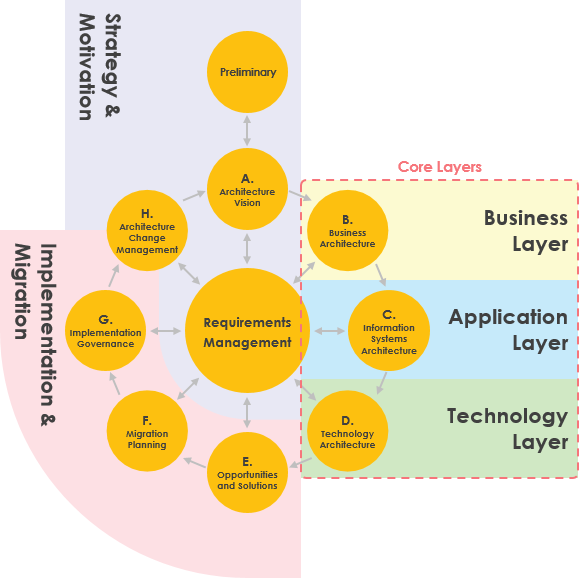
\includegraphics[width=0.8\linewidth]{img/togaf_adm}
	\caption{TOGAF ADM-Zyklus (nach \cite{VisualParadigmTOGAF})}
	\label{fig:togaf_adm}
\end{figure}

Wie zuvor beschrieben stellen die in der Grafik als \textit{Core Layers} bezeichneten Phasen den technischen Entstehungsprozess von IT-Lösungen dar. Die genannte Problematik der Kommunikation zwischen Anwendungs- und Infrastrukturentwicklern liegt hierbei in den Phasen C und D. Phase B wird in dieser Ausarbeitung aus Gründen der Aufgabenstellung vernachlässigt und daher als gegebener aber ebenfalls variabler Teil des Prozesses angesehen. Den Vorteil für die genannte Problematik bietet TOGAF ADM in der Art, wie jede einzelne Phase abgelaufen und wie diese dokumentiert wird \cite{Skript}\cite{TOGAFDocs}.

Jede Phase liefert einen definieren Output, basierend auf einen Input, welcher aus der Phase zuvor hervorgeht und durch phasengetreue Arbeitsschritte erweitert wird. Dieser Output wird auch als "Deliverable" bezeichnet. Während bestimmte Deliverables nur eine kurze Lebensdauer auf sehr begrenzte Phasenabschnitte aufweisen, werden zwei Output-Dokumente von Phase A bis F weitergereicht und be- bzw. überarbeitet. Dabei handelt es sich um das sog. \textit{Architecture Definition Document} (kurz ADD) und die \textit{Architecture Requirements Specification} (kurz ARS). Das ADD beinhaltet hierbei die Dokumentation der operationalen Modelle in unterschiedlichen Abstraktionsgraden und Darstellungsweisen. Die ARS hängt stark mit dem zentralen Requirements Management zusammen und beinhaltet nicht-funktionale Anforderungen unterschiedlicher Problembereiche (bspw. Anforderungen an das laufende System, an Änderungen an das System sowie etwaige Einschränkungen oder Gegebenheiten) \cite{Skript}. Da diese sowie durch die Anwendungsarchitektur (Phase C) sowie die Infrastrukturarchitektur (Phase D) geht, beinhaltet sie detailierte Ausarbeitung aus logischen als auch aus physischen Perspektiven. Diese Sichten betrachten jeweils zwei Zustände: Den Baseline- bzw. Ist-Zustand sowie den gewünschten Target- bzw. Soll-Zustand.  Dadurch sind beide Sichten und Zustände bei korrekter Anwendung des Modells optimal dokumentiert und können in Phase E evaluiert werden, wobei Phase F die Realisierung der Architektur vorsieht, an welcher Stelle die genannten Dokumente ADD und ARS finalisiert und freigegeben werden \cite{TOGAFDocs}\cite{VisualParadigmTOGAF}. Durch das Requirements Management können die jeweiligen Anforderungen von Anwendungs- und Infrastrukturteams ebenfalls frühzeitig erkannt und beachtet werden. Durch die interative Vorgehensweise erlaubt ADM ebenfalls die kontinuierliche, nachträgliche Verbesserung von getätigten Fehlentscheidungen, was ebenfalls vorteilhaft für den Zusammenhand zwischen Anwendungs- und Infrastrukturentwicklung ist. Dadurch ist es auch möglich, im Nachhinein getroffenen Entscheidungen reibungslos in den Prozess einzugliedern. Das könnte sich als vorteilhaft herausstellen, wenn die Architektur letztendlich in eine Public Cloud deployt werden soll.

Ungeachtet dessen beinhaltet ADM ebenfalls die Betrachtung der Implementation-Governance, welche in erster Linie keinen Bezug zur Anwendungs-Infrastruktur-Interdependenz aufweist, jedoch hilfreich und sinnvoll für die weitere Aufgabenstellung erscheint.

Zusammengefasst ist TOGAF ein geeignetes Modell für die gegenwärtigen Gegebenheiten, da es Anwendungsarchitekten und Infrastrukturarchitekten in ihrer Kommunikation unterstützt. Das geschieht über das iterative ADM mit zentralem Anforderungsmanagement sowie der vorteilhaften Dokumentation und Evaluation aller relevanten Sichten und Perspektiven der jeweiligen Beteiligten.